\section{Definitions}
In this section, definitions about graph theory are presented. Most
of the following definitions are taken from or inspired by Wikipedia,
Wikibook and Diestel's Graph Theory book~\cite{Diestel}.

\subsection{Types of graphs}
\paragraph{Undirected simple graphs:}
An undirected simple graph $G$ is a mathematical object composed of a set $V$ of
vertices and a set $E$ of edges and is noted $G = (V,E)$.

%TODO eventually ref for other names in Diestel (nodes/...)
\paragraph{}
An edge is an unordered pair $\{u,v\}$ of vertices and sometimes also denoted 
$uv$ for short.

\paragraph{}
A graph is used to model relation between objects. The vertices represent the 
objects and the edges represent the relation.

\paragraph{}
Thereafter if it is not stated otherwise, a graph refers to an undirected 
simple graphs.


\begin{figure}[!h]
  \begin{center}
    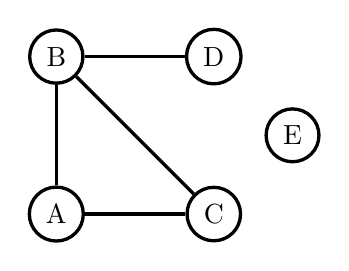
\begin{tikzpicture}[scale=0.5]
  \node[draw,circle, very thick] (A) at (2,0) {A};
  \node[draw,circle, very thick] (B) at (2,4) {B};
  \node[draw,circle, very thick] (C) at (6,0) {C};
  \node[draw,circle, very thick] (D) at (6,4) {D};
  \node[draw,circle, very thick] (E) at (8,2) {E};
  \draw[very thick] (A) -- (B);
  \draw[very thick] (B) -- (D);
  \draw[very thick] (C) -- (B);
  \draw[very thick] (C) -- (A);
\end{tikzpicture}

  \end{center}
  $$V = \{A,B,C,D,E\}$$
  $$E = \Big\{\{A,B\},\{A,C\},\{B,C\},\{B,D\}\Big\}$$
  \caption{An undirected simple graph with 5 vertices and 4 edges}
\end{figure}

\paragraph{Graph Size:}
The size of a graph $G=(V,E)$ is its number of edges, i.e. $|E|$.

\paragraph{Graph order:}
The order of a graph $G=(V,E)$ is its number of vertices, i.e. $|V|$.

\paragraph{Adjacency:}
In a graph $G=(V,E)$, two vertices, $u$ and $v$, are adjacent if $uv \in E$.

\paragraph{Vertex degree:}
The degree of a vertex $v$ in a simple undirected graph is equal to the number of
vertices adjacent to it and it is noted $d(v)$.


\paragraph{Directed graphs:} 
A directed graph is a graph whose edges are defined as ordered pairs
$(u,v)$. The edges of a directed graph are called arcs. 
$u$ is called the head of the arc and $v$ is the tail of the arc.
\begin{figure}[!h]
  \begin{center}
    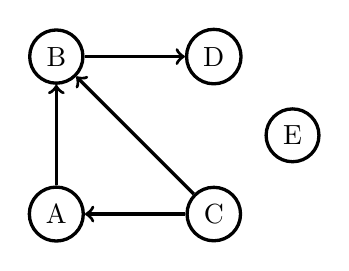
\begin{tikzpicture}[scale=0.5]
 \tikzset{directed/.style={->}} 
  \node[draw,circle, very thick] (A) at (2,0) {A};
  \node[draw,circle, very thick] (B) at (2,4) {B};
  \node[draw,circle, very thick] (C) at (6,0) {C};
  \node[draw,circle, very thick] (D) at (6,4) {D};
  \node[draw,circle, very thick] (E) at (8,2) {E};
  \draw[very thick, directed] (A) -- (B);
  \draw[very thick, directed] (B) -- (D);
  \draw[very thick, directed] (C) -- (B);
  \draw[very thick, directed] (C) -- (A);
\end{tikzpicture}

  \end{center}
  $$V = \{A,B,C,D,E\}$$
  $$E = \Big\{(A,B),(C,A),(C,B),(B,D)\Big\}$$
  \caption{A directed simple graph with 5 vertices and 4 edges}
\end{figure}

\paragraph{Subgraphs:}
Given a graph $G = (V,E)$ and a graph $G' = (V',E')$, then $G'$ is a subgraph of $G$ 
if and only if $V \subseteq V'$ and $E \subseteq E'$.

%TODO to be checked
\paragraph{Induced subgraphs:}
Given a graph $G = (V,E)$ and a set of vertices $V' \subseteq V$, then
there is only one induced subgraph of $G$ by $V'$ and it is denoted
$G' = (V',E')$, with for any pair of vertices $uv$ of $V'$, the edge $uv$ is
in $E'$ if and only if $uv$ is in $E$.

\begin{figure}[!h]
  \begin{center}
    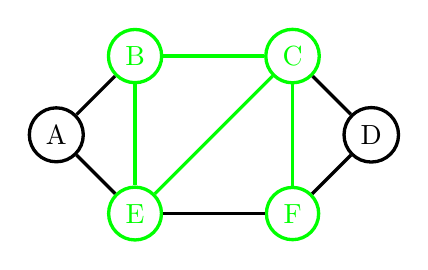
\begin{tikzpicture}[scale=0.5]
  \node[draw,circle, very thick] (A) at (0,2) {A};
  \node[draw,circle, very thick, color=green] (B) at (2,4) {B};
  \node[draw,circle, very thick, color=green] (C) at (6,4) {C};
  \node[draw,circle, very thick] (D) at (8,2) {D};
  \node[draw,circle, very thick, color=green] (E) at (2,0) {E};
  \node[draw,circle, very thick, color=green] (F) at (6,0) {F};
  \draw[very thick] (A) -- (B);
  \draw[very thick] (A) -- (E);
  \draw[very thick, color=green] (B) -- (C);
  \draw[very thick, color=green] (B) -- (E);
  \draw[very thick] (C) -- (D);
  \draw[very thick, color=green] (C) -- (E);
  \draw[very thick, color=green] (C) -- (F);
  \draw[very thick] (D) -- (F);
  \draw[very thick] (E) -- (F);
\end{tikzpicture}

  \end{center}
  \caption{A graph and one of its subgraph (in green)}
\end{figure}

\paragraph{Trees:}
A tree is an undirected simple connected\footnote{See \ref{defConnectivity}}
graph without cycle.

\begin{figure}[!h]
  \begin{center}
    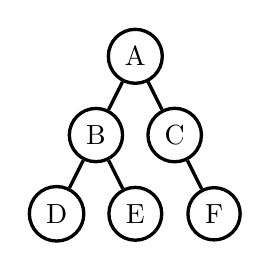
\begin{tikzpicture}[scale=0.5]
  \node[draw,circle, very thick] (A) at (2,4) {A};
  \node[draw,circle, very thick] (B) at (1,2) {B};
  \node[draw,circle, very thick] (C) at (3,2) {C};
  \node[draw,circle, very thick] (D) at (0,0) {D};
  \node[draw,circle, very thick] (E) at (2,0) {E};
  \node[draw,circle, very thick] (F) at (4,0) {F};
  \draw[very thick] (A) -- (B);
  \draw[very thick] (A) -- (C);
  \draw[very thick] (B) -- (D);
  \draw[very thick] (B) -- (E);
  \draw[very thick] (C) -- (F);
\end{tikzpicture}

  \end{center}
  \caption{A tree}
\end{figure}

\paragraph{Root:}
In a tree, one vertex can be distinguished from the other. It is call the root
of the tree.

\paragraph{Descendant:}
Let be $r$ the root of a tree.
Given two vertices $v$ and $w$, if $v$ lies on the unique path between $w$ and 
$r$, then $w$ is a descendant of $v$.

\paragraph{Spanning trees:}
A tree $T$ is a spanning tree of a graph $G$ if it includes every vertex of $G$ 
and is a subgraph of $G$.

\begin{figure}[!h]
  \begin{center}
    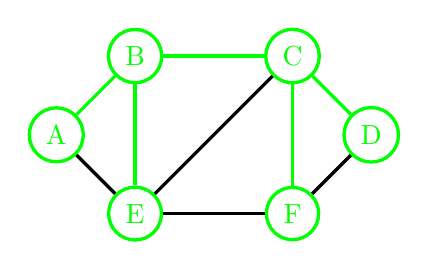
\begin{tikzpicture}[scale=0.5]
  \node[draw,circle, very thick, color=green] (A) at (0,2) {A};
  \node[draw,circle, very thick, color=green] (B) at (2,4) {B};
  \node[draw,circle, very thick, color=green] (C) at (6,4) {C};
  \node[draw,circle, very thick, color=green] (D) at (8,2) {D};
  \node[draw,circle, very thick, color=green] (E) at (2,0) {E};
  \node[draw,circle, very thick, color=green] (F) at (6,0) {F};
  \draw[very thick, color=green] (A) -- (B);
  \draw[very thick] (A) -- (E);
  \draw[very thick, color=green] (B) -- (C);
  \draw[very thick, color=green] (B) -- (E);
  \draw[very thick, color=green] (C) -- (D);
  \draw[very thick] (C) -- (E);
  \draw[very thick, color=green] (C) -- (F);
  \draw[very thick] (D) -- (F);
  \draw[very thick] (E) -- (F);
\end{tikzpicture}

  \end{center}
  \caption{A graph and one of its spanning tree (in green)}
\end{figure}

\paragraph{Complete graphs:}
If all the vertices of $G$ are pairwise adjacent, then $G$ is complete. A
complete graph on $n$ vertices is denoted $K_n$.

\subsection{Paths}
\paragraph{Paths:}
A path is a non-empty graph $P = (V, E)$ of the form
$$ V = \{x_0,x_1, \dots, x_k \} \;\;\; E=\{x_0x_1, x_1x_2, \dots, x_{k-1}x_k \}$$
where the $x_i$ are all distinct. The vertices $x_0$ and $x_k$ are linked
by $P$ and are called its ends; the vertices $x_1, \dots, x_{k-1}$ are the
inner vertices of $P$. The number of edges of path is its
length, and the path of length $k$ is denoted by $P_k$. Note that $k$ is
allowed to be zero; thus, $P_0 = K_1$.

\begin{figure}[!h]
  \begin{center}
    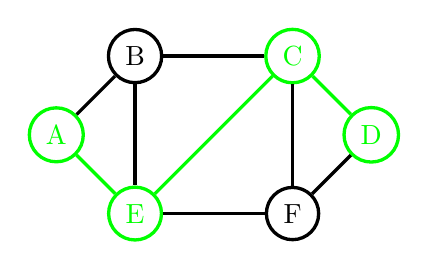
\begin{tikzpicture}[scale=0.5]
  \node[draw,circle, very thick, color=green] (A) at (0,2) {A};
  \node[draw,circle, very thick] (B) at (2,4) {B};
  \node[draw,circle, very thick, color=green] (C) at (6,4) {C};
  \node[draw,circle, very thick, color=green] (D) at (8,2) {D};
  \node[draw,circle, very thick, color=green] (E) at (2,0) {E};
  \node[draw,circle, very thick] (F) at (6,0) {F};
  \draw[very thick] (A) -- (B);
  \draw[very thick, color=green] (A) -- (E);
  \draw[very thick] (B) -- (C);
  \draw[very thick] (B) -- (E);
  \draw[very thick, color=green] (C) -- (D);
  \draw[very thick, color=green] (C) -- (E);
  \draw[very thick] (C) -- (F);
  \draw[very thick] (D) -- (F);
  \draw[very thick] (E) -- (F);
\end{tikzpicture}

  \end{center}
  \caption{A graph and one of its path of length 4 (in green)}
\end{figure}

\paragraph{Vertex-disjoint paths:}
Two paths $P$ and $Q$ are disjoint if and only if they share their ends but
have not any inner vertex in common.

\subsection{Cuts}
Let $G=(V,E)$ be a graph.
\paragraph{Cut:}
A cut $C=(S,T)$ is a partition of $V$ into two subsets $S$ and $T$.

\paragraph{Cut-sets:}
The cut-set of a cut $C=(S,T)$ is the set of edge defined as $\{uv \in E | u \in S \wedge v \in T\}$.

\paragraph{Cut size:}
The size of a cut is the number of edges in the cut-set.

\begin{figure}[!h]
  \begin{center}
    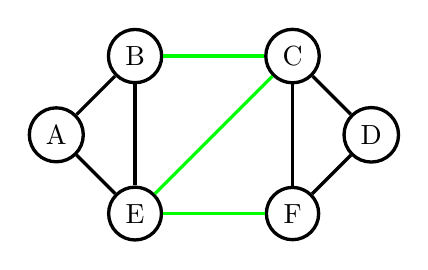
\begin{tikzpicture}[scale=0.5]
  \node[draw,circle, very thick] (A) at (0,2) {A};
  \node[draw,circle, very thick] (B) at (2,4) {B};
  \node[draw,circle, very thick] (C) at (6,4) {C};
  \node[draw,circle, very thick] (D) at (8,2) {D};
  \node[draw,circle, very thick] (E) at (2,0) {E};
  \node[draw,circle, very thick] (F) at (6,0) {F};
  \draw[very thick] (A) -- (B);
  \draw[very thick] (A) -- (E);
  \draw[very thick, color=green] (B) -- (C);
  \draw[very thick] (B) -- (E);
  \draw[very thick] (C) -- (D);
  \draw[very thick, color=green] (C) -- (E);
  \draw[very thick] (C) -- (F);
  \draw[very thick] (D) -- (F);
  \draw[very thick, color=green] (E) -- (F);
\end{tikzpicture}

  \end{center}
  \caption{A graph and one of its cut-set (in green)}
\end{figure}

%\paragraph{Minimum cut:} 
%The minimum cut of a graph G is a cut with the lowest size. 

\paragraph{Articulation set:}
A vertex cut $C$ of a graph $G=(V,E)$ is a subset of $V$ such as the subgraph
of $G$ induced by $V \setminus C$ is disconnected.

\begin{figure}[!h]
  \begin{center}
    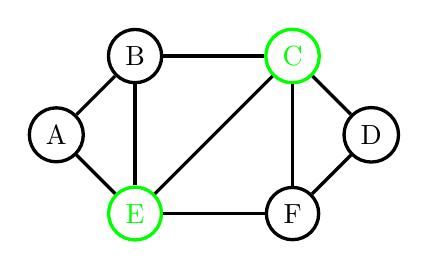
\begin{tikzpicture}[scale=0.5]
  \node[draw,circle, very thick] (A) at (0,2) {A};
  \node[draw,circle, very thick] (B) at (2,4) {B};
  \node[draw,circle, very thick, color=green] (C) at (6,4) {C};
  \node[draw,circle, very thick] (D) at (8,2) {D};
  \node[draw,circle, very thick, color=green] (E) at (2,0) {E};
  \node[draw,circle, very thick] (F) at (6,0) {F};
  \draw[very thick] (A) -- (B);
  \draw[very thick] (A) -- (E);
  \draw[very thick] (B) -- (C);
  \draw[very thick] (B) -- (E);
  \draw[very thick] (C) -- (D);
  \draw[very thick] (C) -- (E);
  \draw[very thick] (C) -- (F);
  \draw[very thick] (D) -- (F);
  \draw[very thick] (E) -- (F);
\end{tikzpicture}

  \end{center}
  \caption{A graph and one of its vertex cut (in green)}
\end{figure}

\subsection{Connectivity}
\paragraph{Connected:}\label{defConnectivity}
A graph $G$ is connected if for every pair $\{u,v\}$ of vertices, there is a 
path from $u$ to $v$. Otherwise, the graph is disconnected.

\paragraph{$k$-connected:}
A graph is $k$-connected if deleting any set of fewer than $k$ vertices do not 
disconnect the graph.

\paragraph{Connectivity:}
The connectivity of a graph is the largest $k$ as it is $k$-connected. 

\begin{figure}[!h]
  \begin{center}
    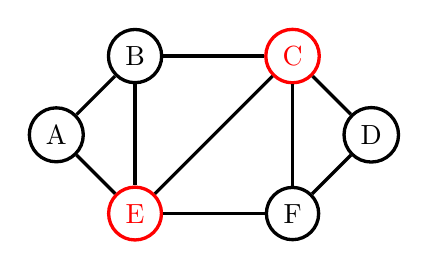
\begin{tikzpicture}[scale=0.5]
  \node[draw,circle, very thick] (A) at (0,2) {A};
  \node[draw,circle, very thick] (B) at (2,4) {B};
  \node[draw,circle, very thick, color=red] (C) at (6,4) {C};
  \node[draw,circle, very thick] (D) at (8,2) {D};
  \node[draw,circle, very thick, color=red] (E) at (2,0) {E};
  \node[draw,circle, very thick] (F) at (6,0) {F};
  \draw[very thick] (A) -- (B);
  \draw[very thick] (A) -- (E);
  \draw[very thick] (B) -- (C);
  \draw[very thick] (B) -- (E);
  \draw[very thick] (C) -- (D);
  \draw[very thick] (C) -- (E);
  \draw[very thick] (C) -- (F);
  \draw[very thick] (D) -- (F);
  \draw[very thick] (E) -- (F);
\end{tikzpicture}

  \end{center}
  \caption{A 2-connected graph}
\end{figure}

\paragraph{Menger's theorem:}
The Menger's theorem is an important theorem concerning connectivity.
It states the following fact:

Let $G$ be a undirected graph and $u$ and $v$ two distinct vertices.
Then the size of the minimum vertex-cut for $u$ and $v$ is equal to the
maximum number of vertex-disjoint paths from $u$ to $v$.

%A graph with at least $k+1$ vertices is $k$-connected, if for every pair {u,v} of
%vertices, there is at least $k$ vertex disjoint paths between these vertices.
%TODO define vertex disjoint paths before
%Another definition could be: a graph is $k$-connex if it's minimal vertex cut
%is of a size less or equal to $k$.


\subsection{Flows}
\paragraph{Flow network}
A flow network is a directed graph $G=(V,E)$ whose edges have a non-negative
capacity, i.e. $\forall (u,v) \in E(G), c(u,v) \geq 0$.

\begin{figure}[!h]
  \begin{center}
    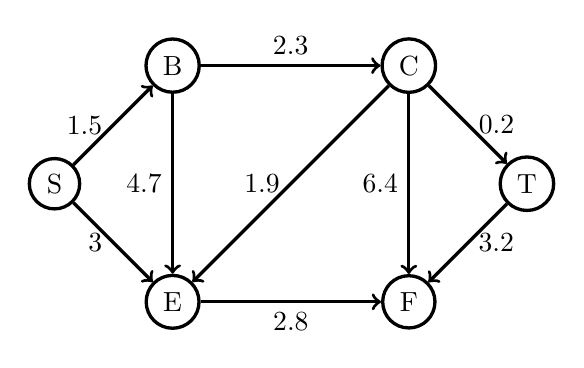
\begin{tikzpicture}[scale=0.5]
 \tikzset{directed/.style={->}} 
  \node[draw,circle, very thick] (A) at (0,3) {S};
  \node[draw,circle, very thick] (B) at (3,6) {B};
  \node[draw,circle, very thick] (C) at (9,6) {C};
  \node[draw,circle, very thick] (D) at (12,3) {T};
  \node[draw,circle, very thick] (E) at (3,0) {E};
  \node[draw,circle, very thick] (F) at (9,0) {F};
  \draw[very thick, directed] (A) -- node[left] {1.5} (B) ;
  \draw[very thick, directed] (A) -- node[left] {3} (E);
  \draw[very thick, directed] (B) -- node[above] {2.3} (C);
  \draw[very thick, directed] (B) -- node[left] {4.7} (E);
  \draw[very thick, directed] (C) -- node[right] {0.2} (D);
  \draw[very thick, directed] (C) -- node[left] {1.9} (E);
  \draw[very thick, directed] (C) -- node[left] {6.4} (F);
  \draw[very thick, directed] (D) -- node[right] {3.2} (F);
  \draw[very thick, directed] (E) -- node[below] {2.8} (F);
\end{tikzpicture}

  \end{center}
  \caption{A flow network}
\end{figure}

\paragraph{Flow:}
Let $G$ be an oriented graph, we distinguish two vertices: a source $s$ and a
sink $t$.
A flow is a function which associates to each edge $(u,v) \in E$ a real:
$f: V \times V \rightarrow \mathbb{R}$ such as:
\begin{itemize}
    \item Capacity constraints: $\forall (u,v) \in E, f(u,v) \leq c(u,v)$
    \item Symetry: $\forall (u,v) \in E, f(u,v) = - f(v,u) $
    \item Flow conservation: $\forall u \in V - \{s,t\}, \sum_{v \in V}f(u,v) = 0$ 
\end{itemize}


%TODO find a ref + reformul the end
\paragraph{Maximum-flow Minimum-cut Theorem:}
The max-flow min-cut theorem~\cite{FD55} states that in a flow network, the maximum amount
of flow passing from the source node to the sink node is equal to the capacity
of the cut which have the minimun capacity.

\subsection{Partitions}
\paragraph{k-partition:}
%TODO redo the def with less math symbol
Let $G = (V,E)$ be a graph,  $\{V_1,...,V_k\}$ is a $k$-partition of $G$, if
and only if:
% With phrases
\begin{itemize}
    \item $\forall i, \lceil V_i \rceil$ is connected
    \item $\sum\limits_{i=0}^k|V_i| = |V|$
    \item $\forall i,j \in \{1, \dots, k\}^2, i \neq j, V_i \cap V_j = \emptyset$
\end{itemize}

\begin{figure}[!h]
    \begin{center}
        
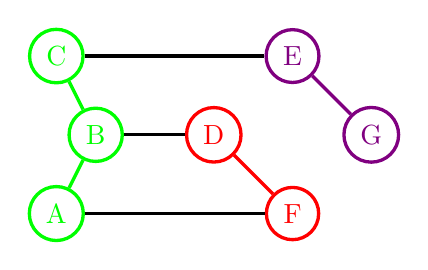
\begin{tikzpicture}[scale=0.5]
  \node[draw,circle, very thick, color=green] (A) at (0,0) {A};
  \node[draw,circle, very thick, color=green] (B) at (1,2) {B};
  \node[draw,circle, very thick, color=green] (C) at (0,4) {C};
  \node[draw,circle, very thick, color=red] (D) at (4,2) {D};
  \node[draw,circle, very thick, color=violet] (E) at (6,4) {E};
  \node[draw,circle, very thick, color=red] (F) at (6,0) {F};
  \node[draw,circle, very thick, color=violet] (G) at (8,2) {G};
  \draw[color=green, very thick] (A) -- (B);
  \draw[color=green, very thick] (B) -- (C);
  \draw[very thick] (B) -- (D);
  \draw[very thick] (A) -- (F);
  \draw[very thick] (C) -- (E);
  \draw[very thick, color=violet] (E) -- (G);
  \draw[very thick, color=red] (D) -- (F);
\end{tikzpicture}

    \end{center}
    \caption{A 3-partition graph}
\end{figure}

